\section{Bill of Materials}
\subsection{Prototype 1 Bill of Materials}
\begin{table}[h]
\begin{tabular}{|cc|c|cc}
\hline
\multicolumn{1}{|c|}{\textbf{Item}}                                                                & \textbf{No.} & \textbf{Total Cost} & \multicolumn{1}{c|}{\textbf{Supplier}} & \multicolumn{1}{c|}{\textbf{Function}}                                                                                                                                                          \\ \hline
\multicolumn{1}{|c|}{\begin{tabular}[c]{@{}c@{}}Arduino\\ MKRWAN1300\end{tabular}}                 & 2            & \$135.04            & \multicolumn{1}{c|}{Arduino}           & \multicolumn{1}{c|}{\begin{tabular}[c]{@{}c@{}}Microcontroller used as\\ LoRaWAN node. \\ Responsible for acceleration\\ and frequency computations, \\ and payload transmission.\end{tabular}} \\ \hline
\multicolumn{1}{|c|}{\begin{tabular}[c]{@{}c@{}}Arduino RF antenna\\ (X000016)\end{tabular}}       & test2        & \$8.74              & \multicolumn{1}{c|}{DigiKey}           & \multicolumn{1}{c|}{\begin{tabular}[c]{@{}c@{}}RF antenna used for LoRa \\ packet transmission.\end{tabular}}                                                                                   \\ \hline
\multicolumn{1}{|c|}{\begin{tabular}[c]{@{}c@{}}Accelerometer\\ (ADXL335)\end{tabular}}            & 1            & \$26.44             & \multicolumn{1}{c|}{DigiKey}           & \multicolumn{1}{c|}{\begin{tabular}[c]{@{}c@{}}Accelerometer used for \\ acceleration sampling.\end{tabular}}                                                                                   \\ \hline
\multicolumn{1}{|c|}{\begin{tabular}[c]{@{}c@{}}Breadboard 400 Tie\\ points (PB8820)\end{tabular}} & 1            & \$8.85              & \multicolumn{1}{c|}{Jaycar}            & \multicolumn{1}{c|}{\begin{tabular}[c]{@{}c@{}}Breadboard used for \\ transmitting node.\end{tabular}}                                                                                          \\ \hline
\multicolumn{1}{|c|}{\begin{tabular}[c]{@{}c@{}}Breadboard 170 \\ points (PB8817)\end{tabular}}    & 1            & \$5.95              & \multicolumn{1}{c|}{Jaycar}            & \multicolumn{1}{c|}{\begin{tabular}[c]{@{}c@{}}Breadboard used for \\ receiving node.\end{tabular}}                                                                                             \\ \hline
\multicolumn{1}{|c|}{AAA battery holder}                                                           & 1            & \$4.50              & \multicolumn{1}{c|}{Jaycar}            & \multicolumn{1}{c|}{\begin{tabular}[c]{@{}c@{}}Battery holder with switch \\ connected to terminal block\\ of the MKRWAN1300.\end{tabular}}                                                     \\ \hline
\multicolumn{1}{|c|}{AAA lithium battery}                                                          & 2            & \$16.95             & \multicolumn{1}{c|}{Jaycar}            & \multicolumn{1}{c|}{\begin{tabular}[c]{@{}c@{}}Powers MKRWAN1300 with\\ total 3.0V.\end{tabular}}                                                                                               \\ \hline
\multicolumn{2}{|c|}{\textbf{Total Cost:}}                                                                        & \textbf{\$206.57}   &                                        &                                                                                                                                                                                                 \\ \cline{1-3}
\end{tabular}
\caption{Prototype 1 Bill of Materials}
\label{proto1-bom}
\end{table}

\subsection{Prototype 2 Bill of Materials}
\begin{table}[H]
\begin{tabular}{|cc|c|cc}
\hline
\multicolumn{1}{|c|}{\textbf{Item}}                                                                                               & \textbf{No.} & \textbf{Total Cost} & \multicolumn{1}{c|}{\textbf{Supplier}}                                               & \multicolumn{1}{c|}{\textbf{Function}}                                                                                       \\ \hline
\multicolumn{1}{|c|}{\begin{tabular}[c]{@{}c@{}}Arduino Maker\\ Subscription\end{tabular}}                                        & 1            & \$10.77             & \multicolumn{1}{c|}{Arduino}                                                         & \multicolumn{1}{c|}{\begin{tabular}[c]{@{}c@{}}Unlimited cloud variables\\ and 3 month data retention.\end{tabular}}         \\ \hline
\multicolumn{1}{|c|}{\begin{tabular}[c]{@{}c@{}}M3 machine screw\\ 20mm\end{tabular}}                                             & 25           & \$4.95              & \multicolumn{1}{c|}{\begin{tabular}[c]{@{}c@{}}Core\\ Electronics\end{tabular}}      & \multicolumn{1}{c|}{\begin{tabular}[c]{@{}c@{}}Used to secure front and \\ back plate of enclosure.\end{tabular}}            \\ \hline
\multicolumn{1}{|c|}{\begin{tabular}[c]{@{}c@{}}M3 machine screw \\ 14mm\end{tabular}}                                            & 25           & \$3.35              & \multicolumn{1}{c|}{\begin{tabular}[c]{@{}c@{}}Core\\ Electronics\end{tabular}}      & \multicolumn{1}{c|}{\begin{tabular}[c]{@{}c@{}}Used to secure lid of \\ enclosure.\end{tabular}}                             \\ \hline
\multicolumn{1}{|c|}{\begin{tabular}[c]{@{}c@{}}Heat-set insert \\ soldering iron tip\end{tabular}}                               & 1            & \$21.88             & \multicolumn{1}{c|}{\begin{tabular}[c]{@{}c@{}}Core \\ Electronics\end{tabular}}     & \multicolumn{1}{c|}{\begin{tabular}[c]{@{}c@{}}Used to install heat-set\\ inserts.\end{tabular}}                             \\ \hline
\multicolumn{1}{|c|}{\begin{tabular}[c]{@{}c@{}}M3 brass heat-set\\ inserts 4mm\end{tabular}}                                     & 50           & \$11.95             & \multicolumn{1}{c|}{\begin{tabular}[c]{@{}c@{}}Core \\ Electronics\end{tabular}}     & \multicolumn{1}{c|}{\begin{tabular}[c]{@{}c@{}}Used to secure front and\\ back plate, and lid of \\ enclosure.\end{tabular}} \\ \hline
\multicolumn{1}{|c|}{\begin{tabular}[c]{@{}c@{}}M2 screw and nut \\ mounting kit\end{tabular}}                                    & 1            & \$23.95             & \multicolumn{1}{c|}{\begin{tabular}[c]{@{}c@{}}Core \\ Electrnoics\end{tabular}}     & \multicolumn{1}{c|}{\begin{tabular}[c]{@{}c@{}}Used to mount PCB in \\ enclosure.\end{tabular}}                              \\ \hline
\multicolumn{1}{|c|}{M10 bolt and nut}                                                                                            & 1            & \$2.68              & \multicolumn{1}{c|}{\begin{tabular}[c]{@{}c@{}}Bunnings\\ Warehouse\end{tabular}}    & \multicolumn{1}{c|}{\begin{tabular}[c]{@{}c@{}}Used to secure enclosure\\ to bridge.\end{tabular}}                           \\ \hline
\multicolumn{1}{|c|}{\begin{tabular}[c]{@{}c@{}}Threadlocker \\ Loctite 10ml\end{tabular}}                                        & 1            & \$15.02             & \multicolumn{1}{c|}{\begin{tabular}[c]{@{}c@{}}Bunnings\\ Warehouse\end{tabular}}    & \multicolumn{1}{c|}{Used to secure all screws.}                                                                              \\ \hline
\multicolumn{1}{|c|}{\begin{tabular}[c]{@{}c@{}}M2 machine screw \\ 30mm\end{tabular}}                                            & 20           & \$8.00              & \multicolumn{1}{c|}{\begin{tabular}[c]{@{}c@{}}Bolt \& Nut\\ Australia\end{tabular}} & \multicolumn{1}{c|}{\begin{tabular}[c]{@{}c@{}}Used to mount PCB in \\ enclosure.\end{tabular}}                              \\ \hline
\multicolumn{1}{|c|}{\begin{tabular}[c]{@{}c@{}}RAKWireless\\ WisGate Edge \\ Lite 2 LoRaWAN\\ Gateway \\ (RAK7268)\end{tabular}} & 1            & \$299.00            & \multicolumn{1}{c|}{\begin{tabular}[c]{@{}c@{}}The IoT \\ Store\end{tabular}}        & \multicolumn{1}{c|}{LoRaWAN gateway.}                                                                                        \\ \hline
\multicolumn{1}{|c|}{PCB}                                                                                                         & 5            & \$13.40             & \multicolumn{1}{c|}{JLCPCB}                                                          & \multicolumn{1}{c|}{\begin{tabular}[c]{@{}c@{}}Carrier board for\\ microcontroller and \\ accelerometer.\end{tabular}}       \\ \hline
\multicolumn{2}{|c|}{\textbf{Total Cost:}}                                                                                                       & \textbf{\$414.95}   &                                                                                      &                                                                                                                              \\ \cline{1-3}
\end{tabular}
\caption{Prototype 2 Bill of Materials}
\label{proto2-bom}
\end{table}

\section{System Diagrams}
\subsection{Python Sender Plotting Script}
\begin{figure}[H]
	\centering
	\caption{Prototype 1 Software Diagram: Sender Plotting}
	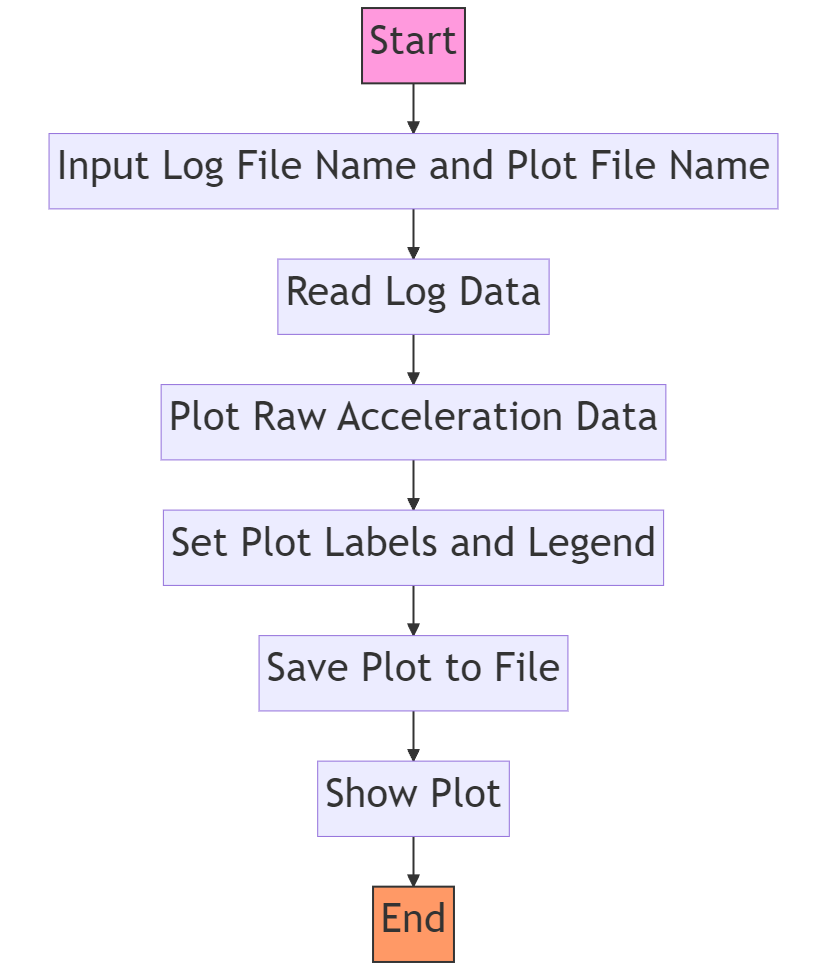
\includegraphics[width=\textwidth]{Sections/Design-Process/proto1-soft-diagram-sender-plot.png}
	\label{proto1-soft-diagram-sender-plot}
\end{figure}

\subsection{Python Receiver Plotting Script}
\begin{figure}[H]
	\centering
	\caption{Prototype 1 Software Diagram: Receiver Plotting}
	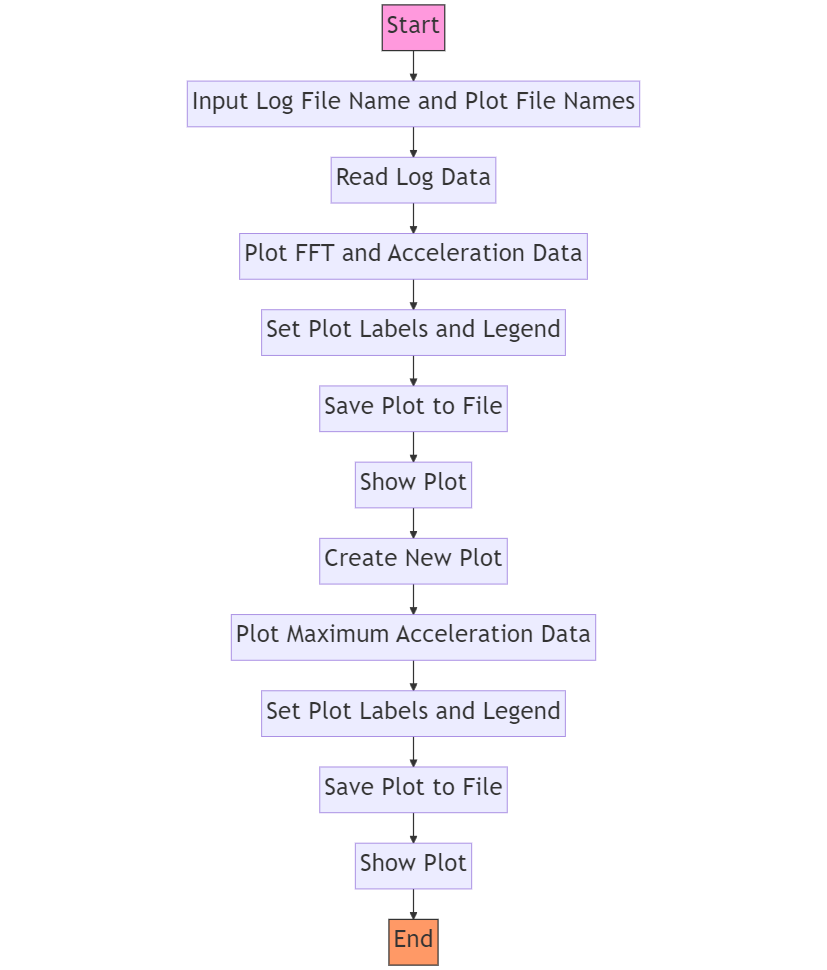
\includegraphics[width=\textwidth]{Sections/Design-Process/proto1-soft-diagram-receiver-plot.png}
	\label{proto1-soft-diagram-receiver-plot}
\end{figure}	

\clearpage
\section{Programs}
\subsection{Prototype 1: Sender Main Program}
\begin{verbatim}
#include "Sender.h"

double xZero = 0.0; double yZero = 0.0; double zZero = 0.0;

void setup() {
  // //Initialise Serial connection
  Serial.begin(9600);
  LoRa.begin(915E6);
  callibrate(256, xZero, yZero, zZero);
}

void loop() {
  // ---------- VARIABLES ----------
  // FFT SAMPLING
  double real_x_axis[sample_n]{}; double imag_x_axis[sample_n]{};
  double real_y_axis[sample_n]{}; double imag_y_axis[sample_n]{};
  double real_z_axis[sample_n]{}; double imag_z_axis[sample_n]{};
  
  // ACCELERATION SAMPLING
  double xAccel[sample_n]{}; double yAccel[sample_n]{}; 
  double zAccel[sample_n]{};

  // VELOCITY SAMPLING
  double xVel[sample_n]{}; double yVel[sample_n]{}; 
  double zVel[sample_n]{};

  // DISPLACEMENT SAMPLING
  double xDisp[sample_n]{}; double yDisp[sample_n]{}; 
  double zDisp[sample_n]{};

  // MAXIMUM ACCELERATION
  double maxAccelX = 0.0; double maxAccelY = 0.0; 
  double maxAccelZ = 0.0;

  // MAXIMUM FREQUENCY
  double xFreq = 0.0; double yFreq = 0.0; double zFreq = 0.0;
  // ---------- VARIABLES ----------

  // ---------- SAMPLE RAW DATA ----------
  readRawData(real_x_axis, real_y_axis, real_z_axis);
  // ---------- SAMPLE RAW DATA ----------
  
  // ---------- TURN RAW DATA INTO ACCELERATION (m/s/s) ----------
  processRawData(xAccel, yAccel, zAccel, real_x_axis, real_y_axis, 
                  real_z_axis, xZero, yZero, zZero);
  // ---------- TURN RAW DATA INTO ACCELERATION (m/s/s) ----------
  
  // ---------- SERIAL PRINT ACCELERATION (m/s/s) ----------
  printAxisValues(xAccel, yAccel, zAccel);
  // ---------- SERIAL PRINT ACCELERATION (m/s/s) ----------

  // ---------- FIND MAX ACCELERATION ----------
  maxAccelX = findMaxAbs(xAccel);
  maxAccelY = findMaxAbs(yAccel);
  maxAccelZ = findMaxAbs(zAccel);
  // ---------- FIND MAX ACCELERATION ----------

  // ---------- REMOVE HIGH FREQUENCIES ----------
  lowPassFilter(xAccel);
  lowPassFilter(yAccel);
  lowPassFilter(zAccel);
  // ---------- REMOVE HIGH FREQUENCIES ----------

  // ---------- COMPUTE FFT ----------
  arduinoFFT xFFT(xAccel, imag_x_axis, sample_n, sampling_rate);
  arduinoFFT yFFT(yAccel, imag_y_axis, sample_n, sampling_rate);
  arduinoFFT zFFT(zAccel, imag_z_axis, sample_n, sampling_rate);

  xFFT.DCRemoval();
  yFFT.DCRemoval();
  zFFT.DCRemoval();

  xFFT.Windowing(window_type, FFT_dir);
  yFFT.Windowing(window_type, FFT_dir);
  zFFT.Windowing(window_type, FFT_dir);

  xFFT.Compute(FFT_dir);
  yFFT.Compute(FFT_dir);
  zFFT.Compute(FFT_dir);

  xFFT.ComplexToMagnitude();
  yFFT.ComplexToMagnitude();
  zFFT.ComplexToMagnitude();
  // ---------- COMPUTE FFT ----------

  // ---------- FIND HIGHEST FREQUENCY ----------
  xFreq = xFFT.MajorPeak();
  yFreq = yFFT.MajorPeak();
  zFreq = zFFT.MajorPeak();
  // ---------- FIND HIGHEST FREQUENCY ----------

  // ---------- CONVERT NAN TO 0 ----------
  checkNan(maxAccelX); 
  checkNan(maxAccelY);
  checkNan(maxAccelZ);

  checkNan(xFreq); 
  checkNan(yFreq);
  checkNan(zFreq);
  // ---------- CONVERT NAN TO 0 ----------

 // ---------- TRANSMIT LORA PACKET ----------
  LoRa.beginPacket();
  LoRa.write((uint8_t*)&xFreq, sizeof(xFreq));
  LoRa.write((uint8_t*)&yFreq, sizeof(yFreq));  
  LoRa.write((uint8_t*)&zFreq, sizeof(zFreq));

  LoRa.write((uint8_t*)&maxAccelX, sizeof(maxAccelX));
  LoRa.write((uint8_t*)&maxAccelY, sizeof(maxAccelY));
  LoRa.write((uint8_t*)&maxAccelZ, sizeof(maxAccelZ));
  LoRa.endPacket();
  // ---------- TRANSMIT LORA PACKET ----------
}
\end{verbatim}

\clearpage
\subsection{Prototype 1: Sender Header File}
\begin{verbatim}
#ifndef Sender_h
#define Sender_h

#include "Arduino.h"
#include <algorithm>
#include <math.h>
#include <MKRWAN.h>
#include <arduinoFFT.h>
#include <LoRa.h>
#include <stdio.h>
#include <iostream> 

static constexpr double pi = 3.14159265358979323846;

//---------- Accelerometer Values ----------
static const int x_axis = A1;
static const int y_axis = A2;
static const int z_axis = A3;
static const int adc_resolution = 4096; //12 BIT ADC
static const double g = 9.81;
const double noiseThreshold = 0.15;
// CALIBRATION
// const double vRef = 3.3; //3.3V reference / supply
const double vRef = 3.0; // BATTERY CONNECTION
static const double sensitivity = 0.33; //330 mV/g at 3.3V
//---------- Accelerometer Values ----------

//---------- FFT Values ----------
static const int frequency = 2;
// THIS IS THE MAXIMUM FREQUENCY THAT THE FFT CAN DETECT
static const int maxFreq = 25; 
static const uint16_t sample_n = 128; //MUST BE EXP 2
// SAMPLING RATE MUST BE AT LEAST TWICE THE MAX FREQUENCY
static const constexpr double sampling_rate = maxFreq * 2; 
 //Gives sample interval in milliseconds
static constexpr double sample_interval = ((1.0/sampling_rate) 
                                            * 1000);

// ---------- FILTER VALUES ----------
constexpr double HP_Fc = 0.5; // high pass cut-off frequency 
constexpr double LP_Fc = 5; // low pass cut-off frequency
constexpr double sampling_period = 1.0 / sampling_rate;

constexpr double HP_alpha = (1 - (2 * pi * HP_Fc 
                                * sampling_period)) 
                            / (1 + (2 * pi * HP_Fc 
                                * sampling_period));
constexpr double LP_alpha = 1 / (1 + (2 * pi * LP_Fc 
                                * sampling_period));

const double alpha = 0.95;
// ---------- FILTER VALUES ----------

//FFT Function Values
// #define window_type FFT_WIN_TYP_HAMMING
#define window_type FFT_WIN_TYP_HANN
#define FFT_dir FFT_FORWARD
//---------- FFT Values ----------

// ---------- FUNCTIONS ----------
double findMaxAbs(const double data[]);
void lowPassFilter(double *data);
void highPassFilter(double *data);
void addGravity(double arr[]);
int findMaxIndex(double arr[]);
double findAvg(double arr[]);
void removeBias(double arr[]);
void integrate(const double arr[], double dt, double integrated[]);
void readRawData(double real_x_axis[], double real_y_axis[], 
                 double real_z_axis[]);
void processRawData(double xAccel[], double yAccel[], 
                    double zAccel[], 
                    const double real_x_axis[], 
                    const double real_y_axis[], 
                    const double real_z_axis[], double xZero, 
                    double yZero, 
                    double zZero);
void integrate(const double xIn[], const double yIn[], 
                const double zIn[], double xOut[], 
                double yOut[], double zOut[]);
// ---------- FUNCTIONS ----------

// ---------- TEST FUNCTIONS ----------
void genSineWave(double arr[]);
void genZeroWave(double arr[]);
void printAxisValues(double xAccel[], double yAccel[], 
                        double zAccel[]);
void printAxisVal(double xFreq, double yFreq, double zFreq);
void printAxisValueSingle(double accel[]);
void callibrate(int callibration_samples, double& xZero, 
                double& yZero, double& zZero);
void checkNan(double& freq);
// ---------- TEST FUNCTIONS ----------

#endif
\end{verbatim}

\subsection{Prototype 1: Sender Functions}

\begin{verbatim}
#include "Sender.h"

void callibrate (int callibration_samples, double& xZero,
                 double& yZero, double& zZero) {
    Serial.println("Calibrating Accelerometer...");

    double offsetX = 0;
    double offsetY = 0;
    double offsetZ = 0;

    for (int i = 0; i < callibration_samples; i++) {
        double rawX = analogRead(x_axis);
        double rawY = analogRead(y_axis);
        double rawZ = analogRead(z_axis);

        double voltageX = (rawX * vRef) / (adc_resolution - 1);
        double voltageY = (rawY * vRef) / (adc_resolution - 1);
        double voltageZ = (rawZ * vRef) / (adc_resolution - 1);

        double accelerationX = (voltageX - vRef / 2) / sensitivity;
        double accelerationY = (voltageY - vRef / 2) / sensitivity;
        double accelerationZ = (voltageZ - vRef / 2) / sensitivity - 1;

        offsetX += accelerationX;
        offsetY += accelerationY;
        offsetZ += accelerationZ;
        delay(10);
    }

    offsetX /= callibration_samples;
    offsetY /= callibration_samples;
    offsetZ /= callibration_samples;

    // ---------- MUST BE TURNED OFF IF PWR IS BATTERY ----------
    // Serial.print("Offset X: ");
    // Serial.println(offsetX, 6);
    // Serial.print("Offset Y: ");
    // Serial.println(offsetY, 6);
    // Serial.print("Offset ccoffsetZ: ");
    // Serial.println(offsetZ, 6);
    // ---------- MUST BE TURNED OFF IF PWR IS BATTERY ----------

    xZero = offsetX;
    yZero = offsetY;
    zZero = offsetZ;
}

double findMaxAbs(const double data[]) {
  double maxVal = 0;
  for (int i = 0; i < sample_n; ++i) {
    double absVal = abs(data[i]);
    if (absVal > maxVal) {
      maxVal = absVal;
    }
  }
  return maxVal;
}

double findMax(const float data[]) {
  double maxVal = 0;
  for (int i = 0; i < sample_n; ++i) {
    double absVal = data[i];
    if (absVal > maxVal) {
      maxVal = absVal;
    }
  }
  return maxVal;
}

void lowPassFilter(double *data) {
  // Initialize with the first value of the data array
  double filteredData = data[0];

  for (uint16_t i = 1; i < sample_n; i++) {
    filteredData = LP_alpha * data[i] + (1.0 - LP_alpha) 
                    * filteredData;
    data[i] = filteredData;
  }
}

double findAvg(double arr[]) {
  double sum = 0.0;
  for (int i = 0; i < sample_n; i++) {
    sum += arr[i];
  }
  return sum / sample_n;
}

void removeBias(double arr[]) { 
  double bias = findAvg(arr);
  for (int i = 0; i < sample_n; i++) {
    arr[i] -= bias;
  }
}

void readRawData(double real_x_axis[], double real_y_axis[], 
                  double real_z_axis[]) {
  for (int i = 0; i < sample_n; i++) {
    // READ RAW DATA FROM ANALOG PINS
    real_x_axis[i] = analogRead(x_axis);
    real_y_axis[i] = analogRead(y_axis);
    real_z_axis[i] = analogRead(z_axis);
    // SAMPLING INTERVAL
    delay(sample_interval);
  }
}

void processRawData(double xAccel[], double yAccel[], 
                    double zAccel[], const double real_x_axis[], 
                    const double real_y_axis[], 
                    const double real_z_axis[], 
                    double xZero, double yZero, double zZero) {
  for (int i = 0; i < sample_n; i++) {
    // CONVERT ADC LEVEL TO A VOLTAGE
    double voltageX = ((real_x_axis[i] * vRef) / (adc_resolution - 1));
    double voltageY = ((real_y_axis[i] * vRef) / (adc_resolution - 1));
    double voltageZ = ((real_z_axis[i] * vRef) / (adc_resolution - 1));

    xAccel[i] = ((voltageX - vRef / 2) / sensitivity - xZero) * g;
    yAccel[i] = ((voltageY - vRef / 2) / sensitivity - yZero) * g;
    // Subtract gravity
    zAccel[i] = ((voltageZ - vRef / 2) / sensitivity - zZero - 1) * g; 

    // // Apply threshold to remove noise
    xAccel[i] = (abs(xAccel[i]) <= 0.7) ? 0 : xAccel[i];
    yAccel[i] = (abs(yAccel[i]) <= 0.9) ? 0 : yAccel[i];
    zAccel[i] = (abs(zAccel[i]) <= 0.1) ? 0 : zAccel[i];
  }
}

void checkNan(float& freq) {
 if (isnan(freq)) {
  freq = 0;
 }
}
\end{verbatim}

\subsection{Prototype 1: Recevier Main Program}
\begin{verbatim}
#include "Receiver.h"

void setup() {
  //Initialise Serial connection
  Serial.begin(9600);
  //Initialise LoRa Connection
  if (!LoRa.begin(915E6)) {
    Serial.println("Starting LoRa failed!");
    while (1);
  }
  Serial.println("LoRa Modem Started");
}

void loop() {
    if (LoRa.parsePacket()) {
    float receivedFreqX;
    float receivedFreqY;
    float receivedFreqZ;

    float receviedAccelX;
    float receviedAccelY;
    float receviedAccelZ;

    LoRa.readBytes((uint8_t*)&receivedFreqX, sizeof(receivedFreqX));
    LoRa.readBytes((uint8_t*)&receivedFreqY, sizeof(receivedFreqY));
    LoRa.readBytes((uint8_t*)&receivedFreqZ, sizeof(receivedFreqZ));

    LoRa.readBytes((uint8_t*)&receviedAccelX, sizeof(receviedAccelX));
    LoRa.readBytes((uint8_t*)&receviedAccelY, sizeof(receviedAccelY));
    LoRa.readBytes((uint8_t*)&receviedAccelZ, sizeof(receviedAccelZ));

    Serial.print(receivedFreqX); 
    Serial.print(" ");
    Serial.print(receivedFreqY);
    Serial.print(" ");
    Serial.print(receivedFreqZ);       

    Serial.print(" ");
    Serial.print(receviedAccelX); 
    Serial.print(" ");
    Serial.print(receviedAccelY);
    Serial.print(" ");
    Serial.println(receviedAccelZ);
  }
}
\end{verbatim}

\subsection{Prototype 1: Sender Logger Program}
\begin{verbatim}
import matplotlib.pyplot as plt
import serial
import time
import os

# MAC ADDRESS
# PORT = '/dev/tty.usbmodem1413301'
# PC ADDERSS
PORT = 'COM3'
BAUD_RATE = 9600
ser = serial.Serial(PORT, BAUD_RATE, timeout=1)

raw_xAccel = []
raw_yAccel = []
raw_zAccel = [] 

fname = input("Enter the name of the log file: ")

def read_serial_data():
    data = ser.readline().decode('utf-8').strip()
    if data:
        variables = data.split(' ')
        if len(variables) == 3 and all(variables):
            try:
                var1, var2, var3 = map(float, variables)
                return var1, var2, var3
            except ValueError:
                print("ERROR: INVALID DATA RECEIVED")
    return None, None, None

print("Ctrl-C to stop logging")

try:
    while True:
        var1, var2, var3 = read_serial_data()
        if var1 is not None and var2 is not None and var3 is not None:
            raw_xAccel.append(var1) 
            raw_yAccel.append(var2)
            raw_zAccel.append(var3)
        time.sleep(0.01)

except KeyboardInterrupt:
    print("Interrupted by user.")

finally:
    # Close the serial port
    ser.close()
    print("Serial port closed.")

# Open and overwrite senderlog
dir_path = "serialPlot/logs/"
full_path = os.path.join(dir_path, fname)

f = open(full_path, "w")
for i in range(len(raw_xAccel)):
    f.writelines([str(raw_xAccel[i]), " ", str(raw_yAccel[i]), \
                    " ", str(raw_zAccel[i]), "\n"])
\end{verbatim}
\subsection{Prototype 1: Sender Plotter Program}
\begin{verbatim}
import matplotlib.pyplot as plt
import time
import os

plt.close('all')

def read_log_data():
    raw_xAccel = []
    raw_yAccel = []
    raw_zAccel = []

    with open(full_path, "r") as f:
        for line in f:
            var1, var2, var3 = map(float, line.split())
            raw_xAccel.append(var1)
            raw_yAccel.append(var2)
            raw_zAccel.append(var3)
    return raw_xAccel, raw_yAccel, raw_zAccel

fname = input("Enter the name of the log file: ")
fname2 = input("Enter the name of the raw acceleration \
               plot file (with file extension): ")

dir_path = "serialPlot/logs/"
full_path = os.path.join(dir_path, fname)

dir_path2 = "serialPlot/plots/"
full_path2 = os.path.join(dir_path2, fname2)

raw_xAccel, raw_yAccel, raw_zAccel = read_log_data()

# Create the plot
plt.plot(raw_xAccel, label="x_axis")
plt.plot(raw_yAccel, label="y_axis")
plt.plot(raw_zAccel, label="z_axis")

# Set plot labels and legend
plt.title("Raw Acceleration")
plt.xlabel("Samples")
plt.ylabel("Acceleration (m/s/s)")
plt.legend()

# Save the figure as a high-resolution PNG file
plt.savefig(full_path2, dpi=300)

# Display the plot
plt.show()
\end{verbatim}
\subsection{Prototype 1: Receiver Logger Program}
\begin{verbatim}
import matplotlib.pyplot as plt
import serial
import time
import os

# MAC ADDRESS
# PORT = '/dev/tty.usbmodem141401'
# PC ADDERSS
PORT = 'COM5'
BAUD_RATE = 9600
ser = serial.Serial(PORT, BAUD_RATE, timeout=1)

xFreq = []
yFreq = []
zFreq = [] 

xAccel = []
yAccel = []
zAccel = []

fname = input("Enter the name of the log file: ")

def read_serial_data():
    data = ser.readline().decode('utf-8').strip()
    if data:
        variables = data.split(' ')
        if len(variables) == 6 and all(variables):
            try:
                var1, var2, var3, var4, var5, var6 = map(float, variables)
                return var1, var2, var3, var4, var5, var6
            except ValueError:
                print("ERROR: INVALID DATA RECEIVED")
    return None, None, None, None, None, None

print("Ctrl-C to stop logging")

try:
    while True:
        var1, var2, var3, var4, var5, var6 = read_serial_data()
        if var1 is not None and var2 is not None and var3 is not None\
            and var4 is not None and var5 is not None and var6 is not None:
            xFreq.append(var1) 
            yFreq.append(var2)
            zFreq.append(var3)

            xAccel.append(var4)
            yAccel.append(var5)
            zAccel.append(var6)
        time.sleep(0.01)

except KeyboardInterrupt:
    print("Interrupted by user.")

finally:
    # Close the serial port
    ser.close()
    print("Serial port closed.")

# Open and overwrite senderlog
dir_path = "serialPlot/logs/"
full_path = os.path.join(dir_path, fname)

f = open(full_path, "w")
for i in range(len(xFreq)):
    f.writelines([str(xFreq[i]), " ", str(yFreq[i]), " ", str(zFreq[i]), \
                  " ", str(xAccel[i]), " ", str(yAccel[i]), \
                    " ", str(zAccel[i]), "\n"]) 
\end{verbatim}
\subsection{Prototype 1: Receiver Plotter Program}
\begin{verbatim}
import matplotlib.pyplot as plt
import serial
import time
import os

plt.close('all')

def read_log_data():
    xVar = []
    yVar = []
    zVar = [] 

    xAccel = []
    yAccel = []
    zAccel = []

    with open(full_path, "r") as f:
        for line in f:
            var1, var2, var3, var4, var5, var6 = map(float, line.split())
            xVar.append(var1)
            yVar.append(var2)
            zVar.append(var3)

            xAccel.append(var4)
            yAccel.append(var5)
            zAccel.append(var6)

    return xVar, yVar, zVar, xAccel, yAccel, zAccel

# Open and overwrite senderlog
fname = input("Enter the name of the log file: ")
fname2 = input("Enter the name of the FFT plot file \
               (with file extension): ")
fname3 = input("Enter the name of the accleration \
               plot file (with file extension): ")

dir_path = "serialPlot/logs/"
full_path = os.path.join(dir_path, fname)

dir_path2 = "serialPlot/plots/"
full_path2 = os.path.join(dir_path2, fname2)

dir_path3 = "serialPlot/plots/"
full_path3 = os.path.join(dir_path3, fname3)

xVar, yVar, zVar, xAccel, yAccel, zAccel = read_log_data()

print("Plotting FFT and Maximum Acceleration")

# Create the plot
plt.plot(xVar, label="x_axis")
plt.plot(yVar, label="y_axis")
plt.plot(zVar, label="z_axis")

# Set plot labels and legend
plt.title("FFT")
plt.xlabel("N's")
plt.ylabel("Frequency (Hz)")
plt.legend()

# Save the figure as a high-resolution PNG file
plt.savefig(full_path2, dpi=300)

# Display the plot
plt.show()

plt.figure()  # Create a new figure for the second plot
plt.plot(xAccel, label="x_axis")
plt.plot(yAccel, label="y_axis")
plt.plot(zAccel, label="z_axis")

# Set plot labels and legend
plt.title("Maximum Acceleration")
plt.xlabel("N's")
plt.ylabel("Max Acceleration (m/s/s)")
plt.legend()

# Save the second figure as a high-resolution PNG files
plt.savefig(full_path3, dpi=300)

# Display the second plot
plt.show()
\end{verbatim}
\subsection{Prototype 2: Sender Main Program}
\begin{verbatim}
#include "arduino_secrets.h"

#include "thingProperties.h"
#include "Sender.h"

double xZero = 0.0; double yZero = 0.0; double zZero = 0.0;
//Store total max values for averaging later
float totalMaxAccelX = 0.0; float totalMaxAccelY = 0.0; 
float totalMaxAccelZ = 0.0;
float totalMaxFreqX = 0.0; float totalMaxFreqY = 0.0; 
float totalMaxFreqZ = 0.0;
//Record the number of computations within the time limit
int computationCount = 0;
//Timing variables
unsigned long previousMillis = 0;
const long interval = 60000; //test scenario 60 seconds

void setup() {
  // Initialize serial and wait for port to open:
  Serial.begin(9600);
  // This delay gives the chance to wait for a Serial Monitor 
  //without blocking if none is found
  delay(1500);

  // Defined in thingProperties.h
  initProperties();

  // Connect to Arduino IoT Cloud
  ArduinoCloud.begin(ArduinoIoTPreferredConnection);
  
  setDebugMessageLevel(2);
  ArduinoCloud.printDebugInfo();
  delay(1500);
  
  callibrate(256, xZero, yZero, zZero);
  delay(1500);
}

void loop() {
  ArduinoCloud.update();

  // ---------- VARIABLES ----------
  double real_x_axis[sample_n] {}; 
  double imag_x_axis[sample_n] {};
  double real_y_axis[sample_n] {}; 
  double imag_y_axis[sample_n] {};
  double real_z_axis[sample_n] {}; 
  double imag_z_axis[sample_n] {};

  // ACCELERATION SAMPLING
  double xAccel[sample_n] {}; double yAccel[sample_n] {}; 
  double zAccel[sample_n] {};

  // MAXIMUM ACCELERATION
  float maxAccelX = 0.0; float maxAccelY = 0.0; 
  float maxAccelZ = 0.0;

  // MAXIMUM FREQUENCY
  float xFreq = 0.0; float yFreq = 0.0; float zFreq = 0.0;
  // ---------- VARIABLES ----------

  // ---------- SAMPLE RAW DATA ----------
  readRawData(real_x_axis, real_y_axis, real_z_axis);
  // ---------- SAMPLE RAW DATA ----------

  // ---------- TURN RAW DATA INTO ACCELERATION (m/s/s) ----------
  processRawData(xAccel, yAccel, zAccel, real_x_axis,
                  real_y_axis, real_z_axis,
                  xZero, yZero, zZero);
  // ---------- TURN RAW DATA INTO ACCELERATION (m/s/s) ----------

  // ---------- SERIAL PRINT ACCELERATION (m/s/s) ----------
  // printAxisValues(xAccel, yAccel, zAccel);
  // ---------- SERIAL PRINT ACCELERATION (m/s/s) ----------

  // ---------- FIND MAX ACCELERATION ----------
  maxAccelX = float(findMaxAbs(xAccel));
  maxAccelY = float(findMaxAbs(yAccel));
  maxAccelZ = float(findMaxAbs(zAccel));
  // ---------- FIND MAX ACCELERATION ----------

  // ---------- REMOVE HIGH FREQUENCIES ----------
  lowPassFilter(xAccel);
  lowPassFilter(yAccel);
  lowPassFilter(zAccel);
  // ---------- REMOVE HIGH FREQUENCIES ----------

  // ---------- COMPUTE FFT ----------
  arduinoFFT xFFT(xAccel, imag_x_axis, sample_n, sampling_rate);
  arduinoFFT yFFT(yAccel, imag_y_axis, sample_n, sampling_rate);
  arduinoFFT zFFT(zAccel, imag_z_axis, sample_n, sampling_rate);

  xFFT.DCRemoval();
  yFFT.DCRemoval();
  zFFT.DCRemoval();

  xFFT.Windowing(window_type, FFT_dir);
  yFFT.Windowing(window_type, FFT_dir);
  zFFT.Windowing(window_type, FFT_dir);

  xFFT.Compute(FFT_dir);
  yFFT.Compute(FFT_dir);
  zFFT.Compute(FFT_dir);

  xFFT.ComplexToMagnitude();
  yFFT.ComplexToMagnitude();
  zFFT.ComplexToMagnitude();
  // ---------- COMPUTE FFT ----------

  // ---------- FIND HIGHEST FREQUENCY ----------
  xFreq = float(xFFT.MajorPeak());
  yFreq = float(yFFT.MajorPeak());
  zFreq = float(zFFT.MajorPeak());
  // ---------- FIND HIGHEST FREQUENCY ----------

  // ---------- CONVERT NAN TO 0 ----------
  checkNan(maxAccelX);
  checkNan(maxAccelY);
  checkNan(maxAccelZ);

  checkNan(xFreq);
  checkNan(yFreq);
  checkNan(zFreq);
  // ---------- CONVERT NAN TO 0 ----------

  totalMaxAccelX += maxAccelX;
  totalMaxAccelY += maxAccelY;
  totalMaxAccelZ += maxAccelZ;

  totalMaxFreqX += xFreq;
  totalMaxFreqY += yFreq;
  totalMaxFreqZ += zFreq;

  computationCount++;

  unsigned long currentMillis = millis();
  if (currentMillis - previousMillis >= interval) {
    previousMillis = currentMillis;

    float averageMaxAccelX = totalMaxAccelX / computationCount;
    float averageMaxAccelY = totalMaxAccelY / computationCount;
    float averageMaxAccelZ = totalMaxAccelZ / computationCount;

    float averageMaxFreqX = totalMaxFreqX / computationCount;
    float averageMaxFreqY = totalMaxFreqY / computationCount;
    float averageMaxFreqZ = totalMaxFreqZ / computationCount;

    Serial.print(averageMaxAccelX);
    Serial.print(" ");
    Serial.print(averageMaxAccelY);
    Serial.print(" ");
    Serial.print(averageMaxAccelZ);
    Serial.print(" ");
    Serial.print(averageMaxFreqX);
    Serial.print(" ");
    Serial.print(averageMaxFreqY);
    Serial.print(" ");
    Serial.println(averageMaxFreqZ);

    dev1_cloud_avg_max_accel_x = averageMaxAccelX;
    dev1_cloud_avg_max_accel_y = averageMaxAccelY;
    dev1_cloud_avg_max_accel_z = averageMaxAccelZ;

    dev1_cloud_avg_max_freq_x = averageMaxFreqX;
    dev1_cloud_avg_max_freq_y = averageMaxFreqY;
    dev1_cloud_avg_max_freq_z = averageMaxFreqZ;

    totalMaxAccelX = 0.0;
    totalMaxAccelY = 0.0;
    totalMaxAccelZ = 0.0;

    totalMaxFreqX = 0.0;
    totalMaxFreqY = 0.0;
    totalMaxFreqZ = 0.0;

    computationCount = 0;
  }
}
\end{verbatim}
\subsection{Prototype 2: Sender Thing Properties Header File}
\begin{verbatim}
// Code generated by Arduino IoT Cloud, DO NOT EDIT.

#include <ArduinoIoTCloud.h>
#include <Arduino_ConnectionHandler.h>


const char THING_ID[] = "09f4b4cd-c539-49df-9701-d4c915b536ae";

const char APPEUI[]   = SECRET_APP_EUI;
const char APPKEY[]   = SECRET_APP_KEY;


float dev1_cloud_avg_max_accel_x;
float dev1_cloud_avg_max_accel_y;
float dev1_cloud_avg_max_accel_z;
float dev1_cloud_avg_max_freq_x;
float dev1_cloud_avg_max_freq_y;
float dev1_cloud_avg_max_freq_z;

void initProperties(){
  ArduinoCloud.setThingId(THING_ID);
  ArduinoCloud.addProperty(dev1_cloud_avg_max_accel_x, 1,
                            READ, ON_CHANGE, NULL);
  ArduinoCloud.addProperty(dev1_cloud_avg_max_accel_y, 2,
                            READ, ON_CHANGE, NULL);
  ArduinoCloud.addProperty(dev1_cloud_avg_max_accel_z, 4,
                            READ, ON_CHANGE, NULL);
  ArduinoCloud.addProperty(dev1_cloud_avg_max_freq_x, 5, 
                            READ, ON_CHANGE, NULL);
  ArduinoCloud.addProperty(dev1_cloud_avg_max_freq_y, 7, 
                            READ, ON_CHANGE, NULL);
  ArduinoCloud.addProperty(dev1_cloud_avg_max_freq_z, 8, 
                            READ, ON_CHANGE, NULL);

}

LoRaConnectionHandler ArduinoIoTPreferredConnection(APPEUI,  
      APPKEY, _lora_band::AU915, "ff000001f000ffff00020000");
\end{verbatim}

\section{Network Layer}
\subsection{TNN Live Data}
\begin{figure}[H]
	\centering
	\caption{TNN Live Data View}
	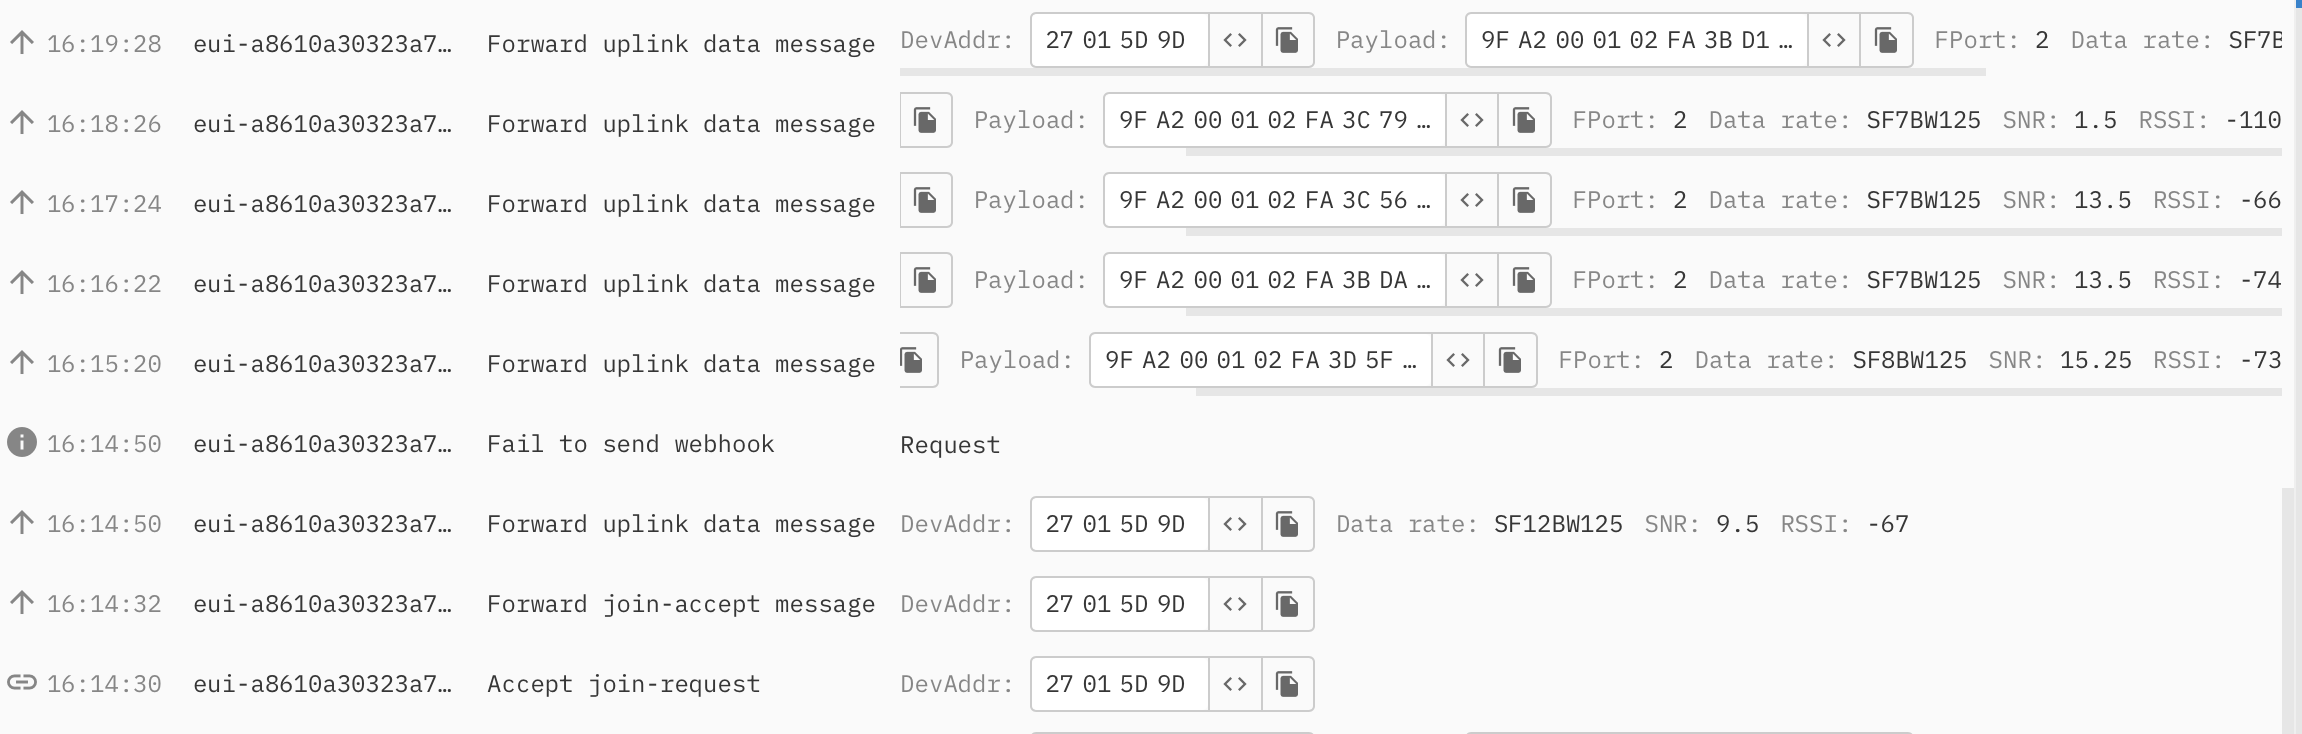
\includegraphics[width=\textwidth]{Sections/Appendix/TNN-live.png}
	\label{tnn-live}
\end{figure}

\subsection{Arduino Iot Cloud Dashboard}
\begin{figure}[H]
	\centering
	\caption{Arduino IoT Cloud Dashboard Desktop View}
	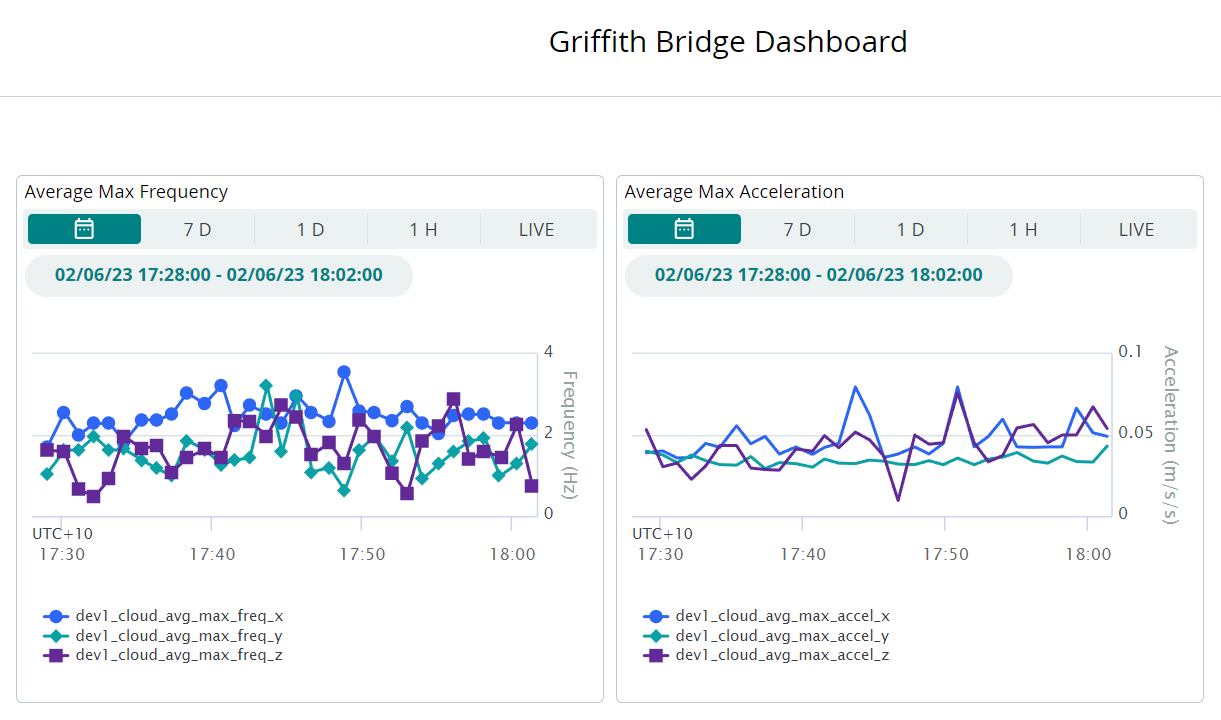
\includegraphics[width=\textwidth]{Sections/Appendix/dashboard.png}
	\label{dashboard}
\end{figure}

\begin{figure}[H]
	\centering
	\caption{Arduino IoT Cloud Dashboard Phone View}
	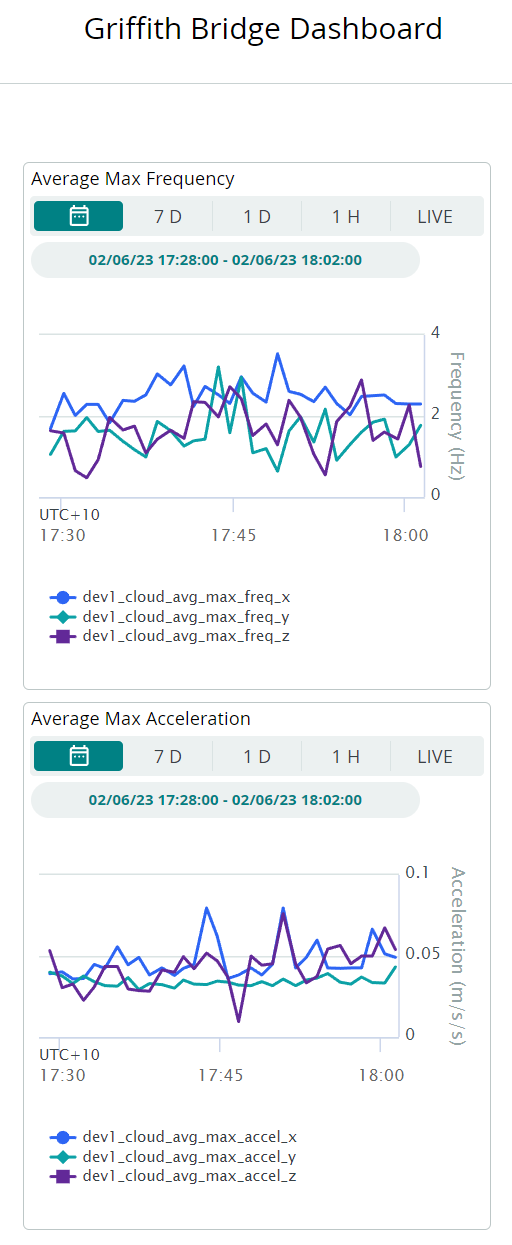
\includegraphics[scale=0.6]{Sections/Appendix/dashboard-phone.png}
	\label{dashboard-phone}
\end{figure}